%! Author = adnansiddiquei
%! Date = 19/03/2024

\section{Custom Degradation - Gaussian Blur}\label{sec:q2}
A Gaussian blur degradation was implemented to train a diffusion model on the MNIST dataset.
This section discusses the design of this model, the training process and a comparison of this model with the 3 models
trained in Section~\eqref{sec:q1bc}.

\subsection{Model Design}\label{subsec:model-design}
\begin{figure}[t]
    \centering
    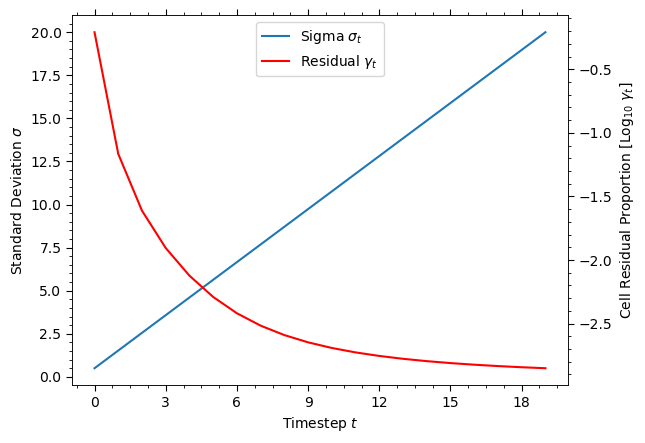
\includegraphics[width=0.8\textwidth]{figures/q2_blur_schedule}
    \caption{A plot of the blur schedule for the Gaussian blur mode.
        The blue line shows how the standard deviation of the Gaussian blur changes across timesteps (left axis).
        The red line shows the proportion of the original cell's value that is retained in the blurred cell (computed from
        the 1 cell central area of the 2D Gaussian kernel with a kernel size of 29).
        The right axis is in log scale and is termed $\gamma_{t}$.}
    \label{fig:q2_blur_schedule}
\end{figure}

The exact same CNN architecture was used as in Section~\eqref{sec:q1bc} to learn the diffusion process.
The primary differences were the \inlinecode{forward} and \inlinecode{sample} functions, with the sampling process
derived from Bansal et al., (2022)~\cite{bansal}.

The forward function worked in a similar way to the \inlinecode{DDPM} models.
A random timestep $t$ was sampled in the range $[1, 20]$ and a Gaussian blur was applied to the MNIST image using
\inlinecode{torchvision.transforms.GaussianBlur} with a kernel size of 29 and a standard deviation of according to the
linear "blur schedule" shown in Figure~\eqref{fig:q2_blur_schedule}.
As displayed in the figure, the standard deviation of the Gaussian blur increased linearly with time, resulting in a
exponentially blurred image as the timestep increased.
Given that the \inlinecode{GaussianBlur} function 0-pads on the edge, the images were scaled to $[0, 1]$ to ensure that
0 represented black cells.
The loss function was an \inlinecode{nn.MSELoss}, with arguments being the original image and the blurred image, and the
model was trained using the MNIST training set.
All other hyperparameters (epochs, optimiser, learning rate) were kept the same as in Section~\eqref{sec:q1bc}.

Conditional sampling was used for the sampling process where a random MNIST digit from the test set was blurred to the
final timestep, and the model was used to reverse the blurred image back to a new image by using Algorithm 2 from
Bansal et al., (2022)~\cite{bansal}.

\subsection{Model Training}\label{subsec:model-training}
